\begin{enunciado}{\ejercicio[MergeSelectivo*Hacer*]}
  \textit{MergeSelectivo}

  Dados dos arreglos de naturales, ambos ordenados de manera creciente, se desea buscar, dada una posición $i$,
  el $i-$ésimo elemento de la unión de ambos. Dicho de otra forma, el $i-$ésimo del resultado de hacer merge ordenado
  entre ambos arreglos. Notar que no es necesario hacer el merge completo. Se puede asumir que cada natural
  aparece a lo sumo en uno de los arreglos, y a lo sumo una vez.
  \begin{enumerate}[label=\arabic*)]
    \item Implementar al función \textit{iésimoMerge} que dados los arreglos $A$ y $B$, y un valor $i$ natural, resuelva
          el problema planteado.

    \item Calcular y justificar la complejidad del algoritmo propuesto. La complejidad temporal debe ser $O(\log^2n)$,
          dónde $n = |A| = |B|$. \textbf{Hint:} Observar que, dado el valor de un elemento de alguno de los dos arreglos, se puede
          averiguar en tiempo $O(\log(n))$ entre qué par de posiciones consecutivas del otro arreglo quedaría, y de allí deducir
          cuál sería la posición en el merge.

    \item \textbf{Desafío adicional:} Intente resolver el mismo problema en tiempo $O(\log n)$ (este ítem es bastante más
          difícil).
  \end{enumerate}
\end{enunciado}

\begin{enumerate}[label=\arabic*]
    \item Hecho junto al 2.
    \item La idea es la siguiente: dado i, sabemos que el i-esimo elemento del merge está en el array A o en el array B.
          De modo que comenzamos buscando si está en el array A y si no está buscamos en el array B.
          Para buscar si está en el array lo que hacemos es una especie de búsqueda binaria, calculando para los elementos su posición en el merge.
          Esto último lo hacemos con la sugerencia del enunciado, con lo que tendriamos una búsqueda binaria dentro de otra,
          lo cual esperamos que de el $O(\log^{2}(n))$ deseado. 
          
          
          \lstset{
          mathescape=true,
          emph={[1]funcion, return, ret, retorno},
          emph={[2]for,each, si, sino, if, else, true, false, not},
          emph={[3]cazadorDeFalsos, conjuncionSubmatriz},
          emphstyle={[1]\color{violet}\it},
          emphstyle={[2]\color{red}\it},
          emphstyle={[3]\color{OliveGreen}\it},
          morecomment={[l]{//}},
          commentstyle={\color{gray}\it\footnotesize}
        }
        \begin{tcolorbox}
          \begin{lstlisting}
funcion iesimoMerge(A, B, i)     // 0<= i <|A|+|B|
    res = buscar(A, B, i, 0, |A|-1)
    si res != false
        ret res
    sino
        ret buscar(B, A ,i ,0 , |B|-1)       // Como no está en A, buscamos en B

funcion buscar(A, B, i, izq, der)            // Devuelve, si está, el elemento de A que está en el i-esimo lugar en el merge 
    si izq > der
      ret false                           // No está en el array

    medio = (izq+der)/2
    
    posMedio = posMerge(B, A[medio], medio, 0, |A|-1)
    
    si posMedio = i
      ret A[medio]
    else if posMedio > i
      ret buscar(A, B, i, izq, medio-1)
    else
      ret buscar(A, B, i, medio+1, der)

funcion posMerge(B, e, j, izq, der)        // Dado e y su posición j en el array, devuelve la posicion que tiene en el merge
    si izq > der
      ret j + izq             // La suma de la cantidad de elementos menores a e en cada array

    medio = (izq+der)/2

    if B[medio] > e
      ret posMerge(B, e, j, izq, medio-1)
    else
      ret posMerge(B, e, j, medio +1 , der)
\end{lstlisting}
        \end{tcolorbox}

        Como no hay repetidos no nos preocupamos por si va un $>$ o $>=$ durante las recursiones.

        Ahora analicemos la complejidad. La complejidad de \textit{posMerge} es igual al de búsqueda binaria: $O(log(n))$ 
        con $n = der - izq + 1$. En el caso de \textit{buscar} obtenemos la siguiente recursión:

        $$
          T(n) =
          \llave{ccl}{
            1 & \text{si} & n = 1  \\
            T(n/2) + \log(n) & \text{si} & n > 1
          }
        $$

        Observamos que no se puede resolver con el teorema Maestro, pues $\log(n)$ no es superior que $n^{\epsilon}$ para ningún $\epsilon >0$.
        Con lo que suponemos $n$ potencia de 2 y armamos árbol:

        \begin{center}
            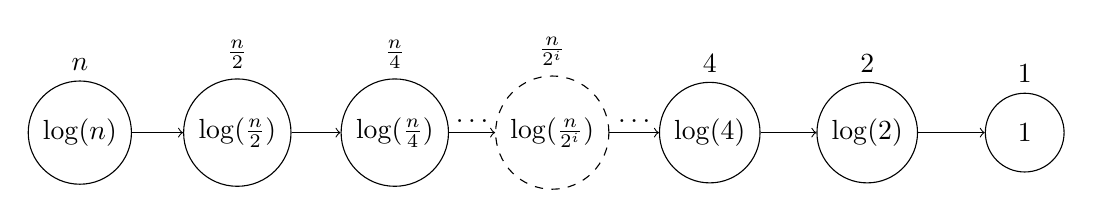
\begin{tikzpicture}[node distance=2cm]

                  \node[circle, draw, minimum size=1cm, label=above:{$n$}] (n0) {$\log(n)$};
                  \node[circle, draw, minimum size=1cm, right of=n0, label=above:{$\frac{n}{2}$}] (n1) {$\log(\frac{n}{2})$};
                  \node[circle, draw, minimum size=1cm, right of=n1, label=above:{$\frac{n}{4}$}] (n2) {$\log(\frac{n}{4})$};
                  \node[circle, draw, minimum size=1cm, right of=n2, dashed, label=above:{$\frac{n}{2^i}$}] (ndots) {$\log(\frac{n}{2^i})$};
                  \node[circle, draw, minimum size=1cm, right of=ndots, label=above:{$4$}] (n3) {$\log(4)$};
                  \node[circle, draw, minimum size=1cm, right of=n3, label=above:{$2$}] (n4) {$\log(2)$};
                  \node[circle, draw, minimum size=1cm, right of=n4, label=above:{$1$}] (n5) {$1$};

                  \draw[->] (n0) -- node[above] {} (n1);
                  \draw[->] (n1) -- node[above] {} (n2);
                  \draw[->] (n2) -- node[above] {$\dots$} (ndots);
                  \draw[->] (ndots) -- node[above] {$\dots$} (n3);
                  \draw[->] (n3) -- node[above] {} (n4);
                  \draw[->] (n4) -- node[above] {} (n5);

            \end{tikzpicture}
        \end{center}
             
        De este modo, la complejidad está dada por:

        $$
          \sumatoria{i=0}{\log(n) - 1} \log(\frac{n}{2^i}) = \sumatoria{i=0}{\log(n) - 1} \log(n) - i = \log(n)\log(n) - \frac{(\log(n)-1)\log(n)}{2} = \frac{\log^2(n)}{2} + \frac{\log(n)}{2} = O(\log^2(n))
        $$

        Finalmente se observa que \textit{iesimoMerge} en el peor caso llama dos veces a esta función, de modo que efectivamente la complejidad es 
        $\cajaResultado{O(\log^2(n))}$


    \item \hacer
\end{enunciado}